\section*{Appendix}
\addcontentsline{toc}{section}{Appendix}

\subsection{Web-Based Platform for Data Partitioning Evaluation}\label{subsec:web_platform}

\begin{figure*}[h]
    \centering
    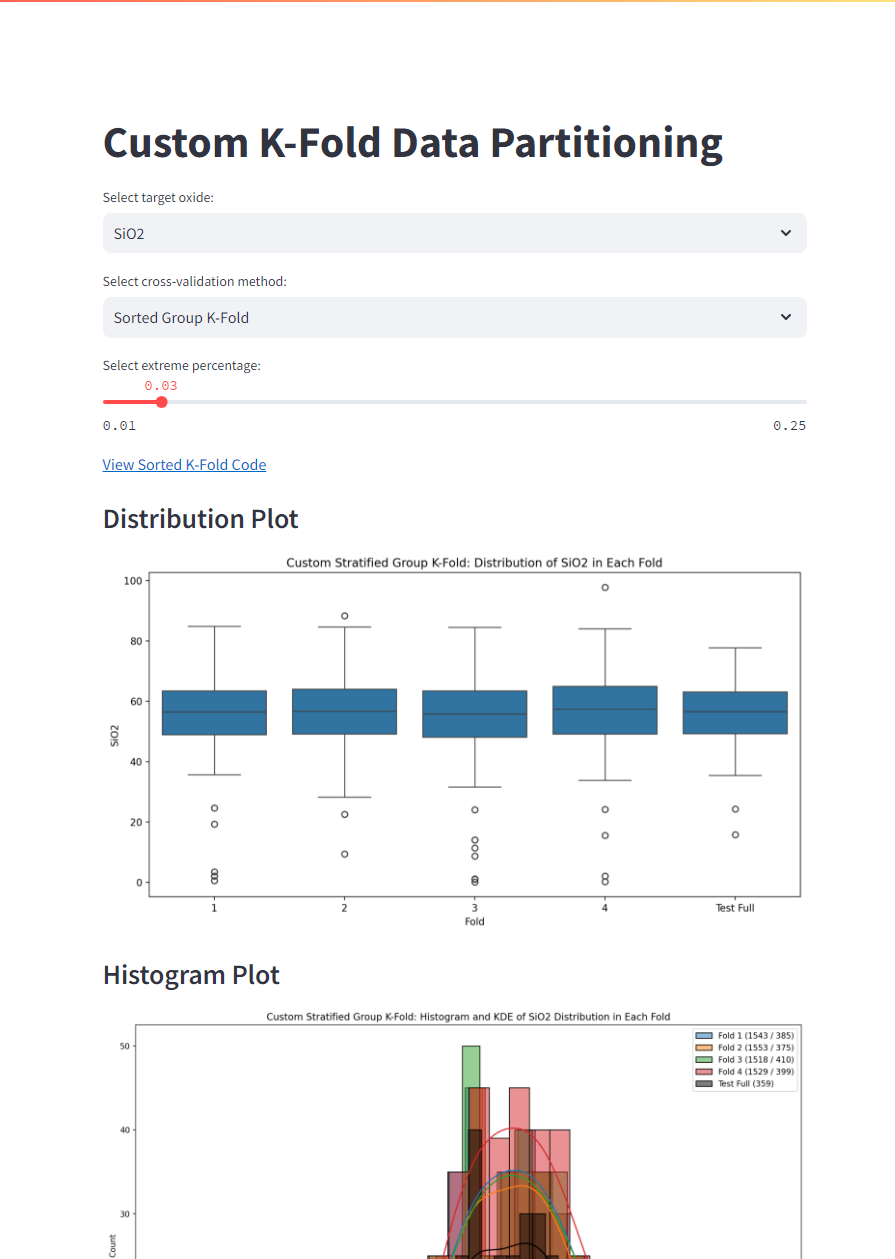
\includegraphics[width=\textwidth]{images/web_platform.png}
    \caption{Web-based platform used to determine the optimal value of $p$ for the data partitioning algorithm.}
    \label{fig:web_platform}
\end{figure*}

\subsection{Cross-Validation Plots for Major Oxides}\label{subsec:cv_plots}

% Loop through each major oxide and add a subsubsection with figures
\foreach \oxide in {SiO2, TiO2, Al2O3, FeOT, MgO, CaO, Na2O, K2O} {
    \subsubsection{\oxide}

    \begin{figure*}[h!]
        \centering
        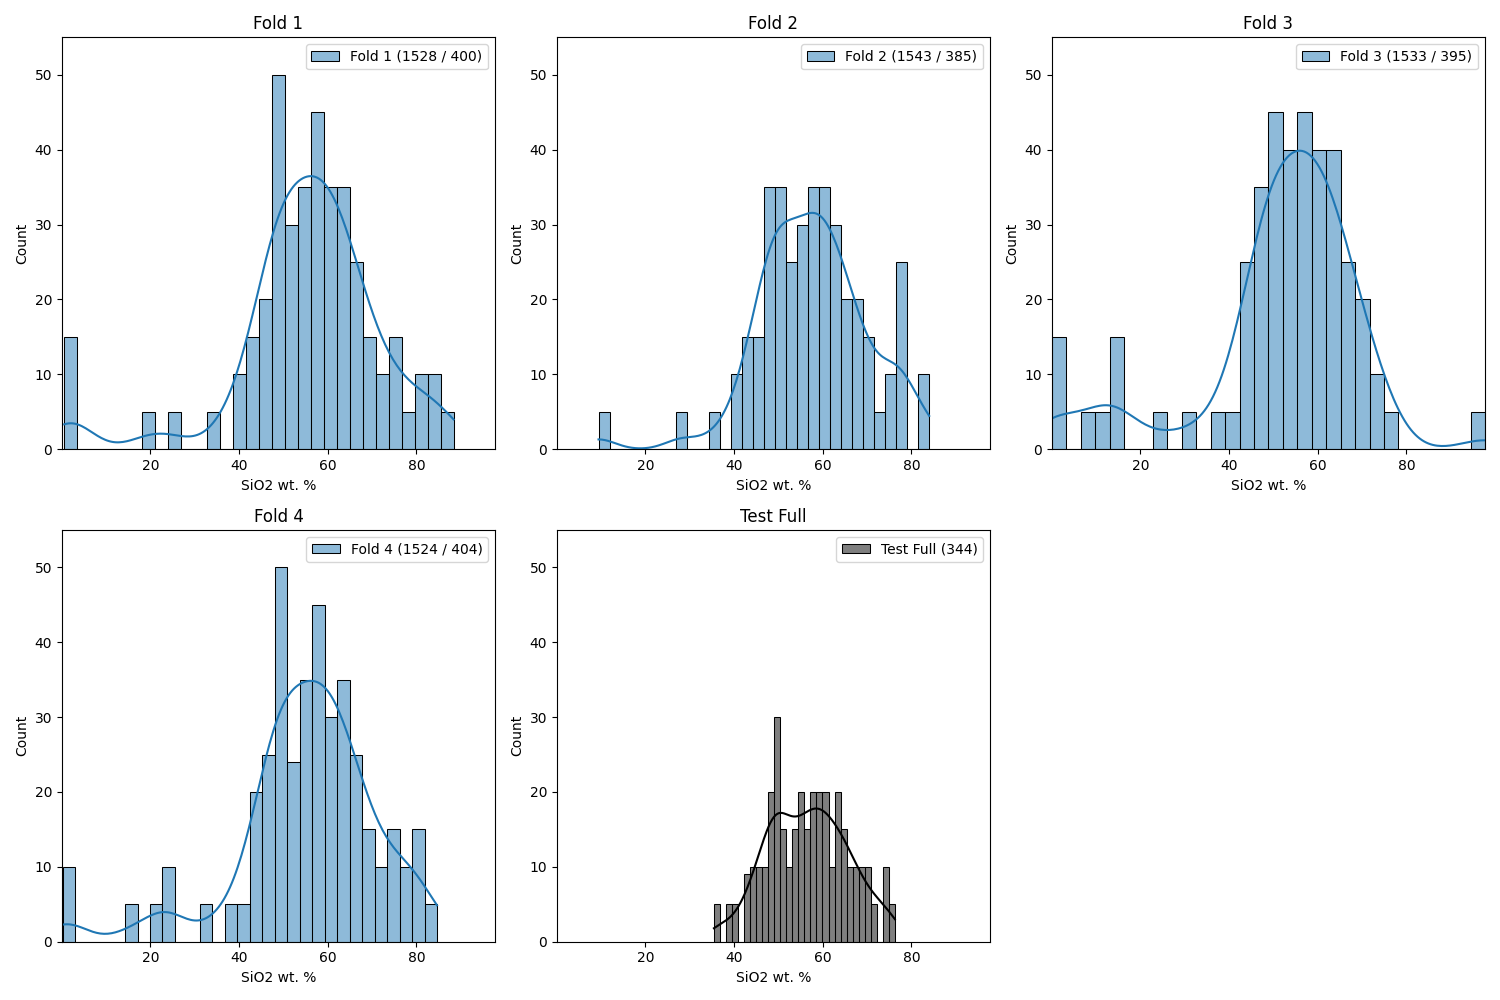
\includegraphics[width=\textwidth]{images/\oxide/histogram_grid_plot.png}
        \caption{Histogram and \gls{kde} of \ce{\oxide} distribution in each fold. The y-axis represents the count of samples per bin, and the x-axis represents \ce{\oxide} concentration. The notation in the legend indicates the amount of instances in the training/validation sets.}
        \label{fig:histogram_grid_plot_\oxide}
    \end{figure*}

    \begin{figure*}[h!]
        \centering
        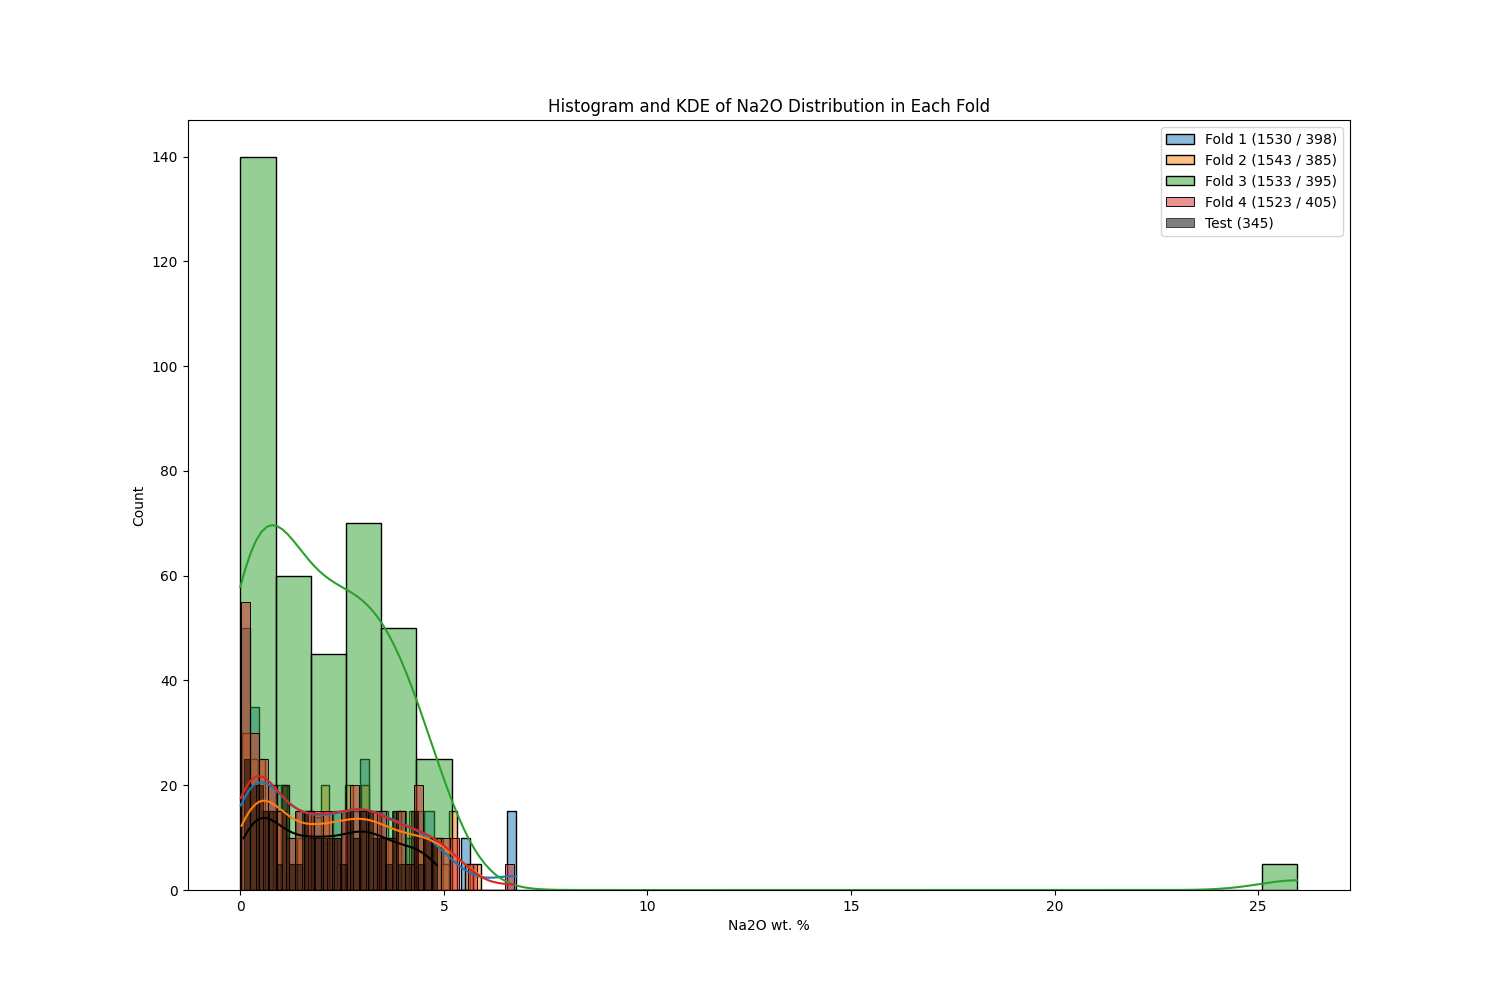
\includegraphics[width=\textwidth]{images/\oxide/histogram_kde_plot.png}
        \caption{Combined Histogram and \gls{kde} of \ce{\oxide} distribution in each fold. The y-axis represents the count of samples per bin, and the x-axis represents \ce{\oxide} concentration. The notation in the legend indicates the amount of instances in the training/validation sets.}
        \label{fig:histogram_kde_plot_\oxide}
    \end{figure*}

    \begin{figure*}[h!]
        \centering
        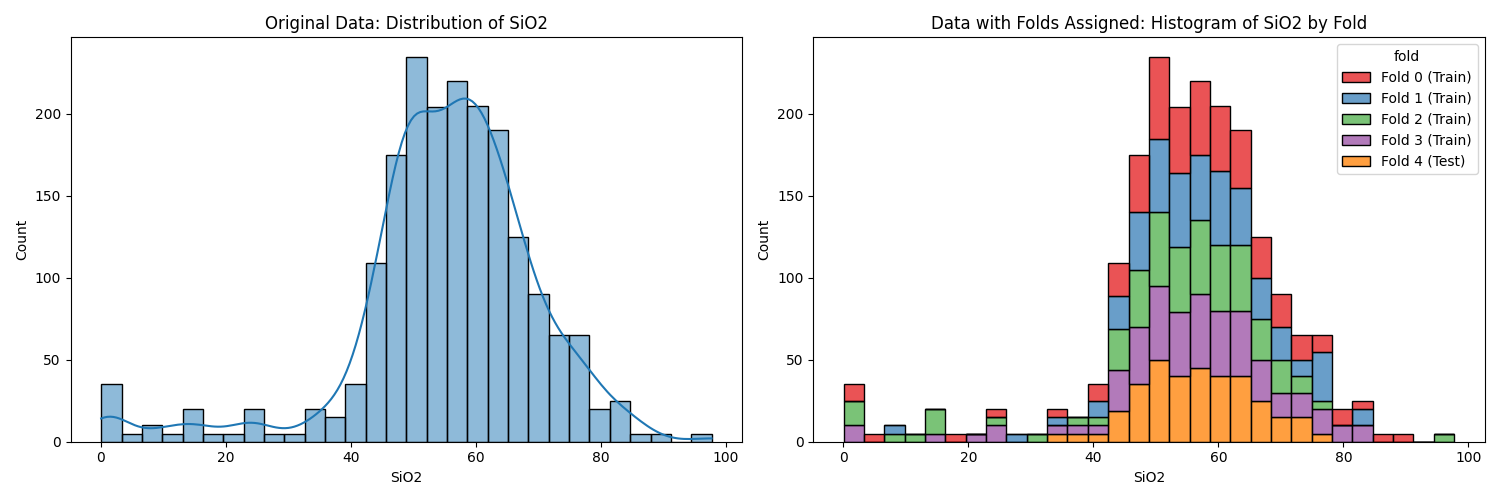
\includegraphics[width=\textwidth]{images/\oxide/original_and_post_fold.png}
        \caption{Distribution of \ce{\oxide} concentrations before and after fold assignment. The left plot shows the original distribution of \ce{\oxide}, while the right plot shows the distribution with folds assigned, color-coded to indicate the different folds.}
        \label{fig:original_and_post_fold_plot_\oxide}
    \end{figure*}

    \begin{figure*}[htbp]
        \centering
        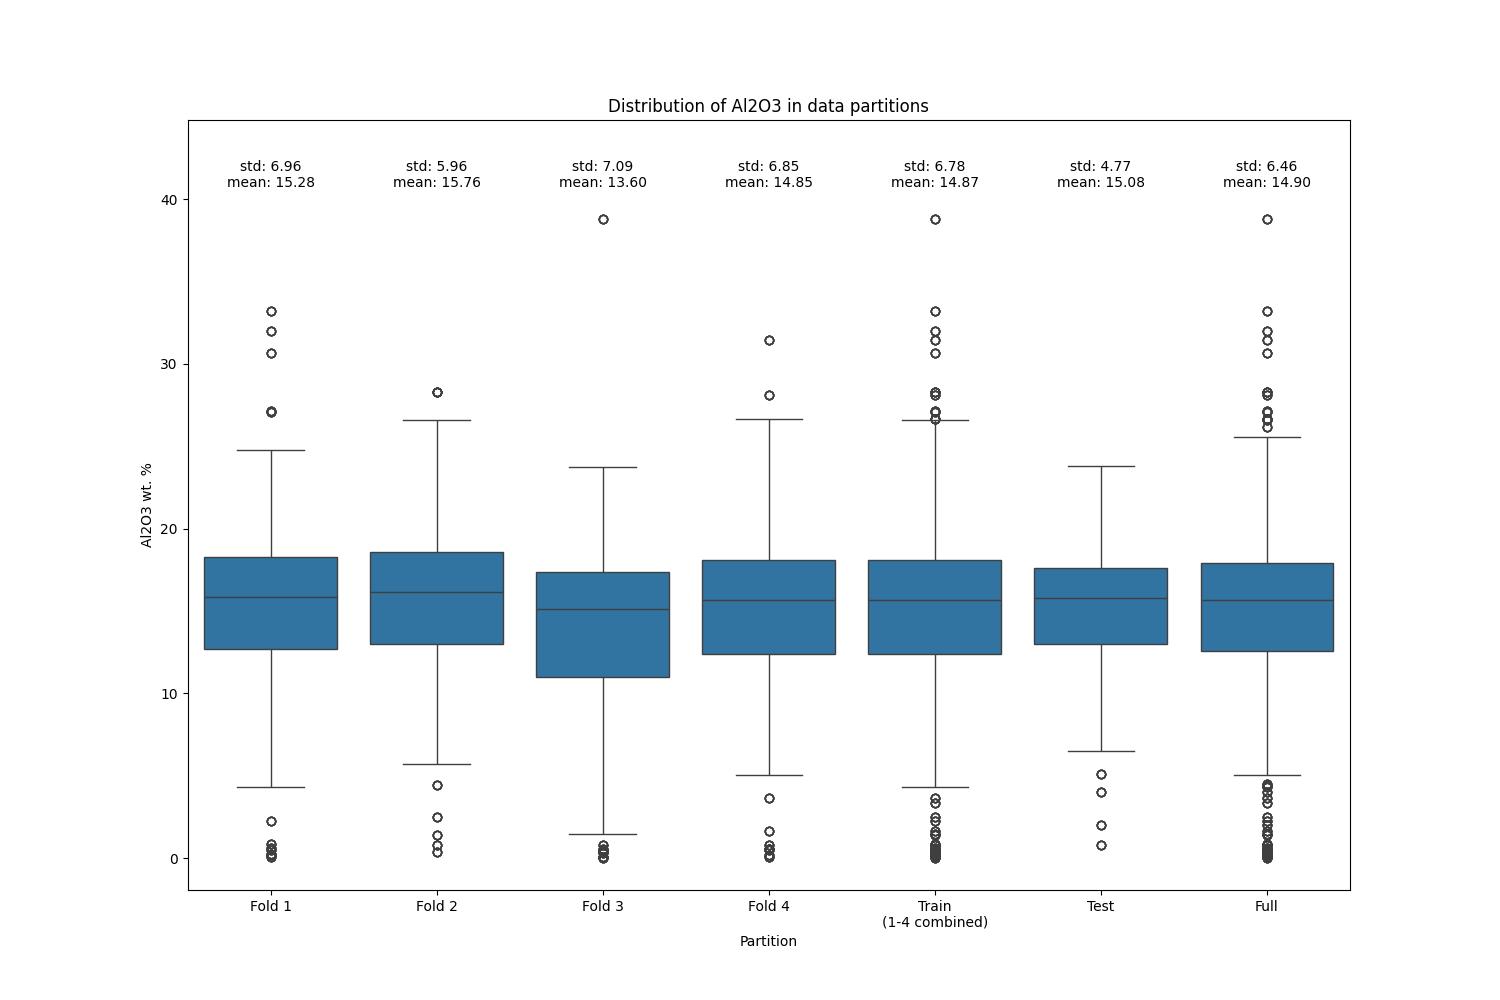
\includegraphics[width=\textwidth]{images/\oxide/distribution_plot.png}
        \caption{Distribution of \ce{\oxide} concentrations across cross-validation folds, training set, test set, and the entire dataset. The mean and standard deviation statistics for each partition are indicated figure.}
        \label{fig:distribution_plot_\oxide}
    \end{figure*}
}